\documentclass[11pt,titlepage]{article}

%\usepackage[cp1250]{inputenc}
%\usepackage[czech]{babel}
%\usepackage[top=1.5cm, bottom=1.5cm, left=1.5cm, right=1.5cm]{geometry}
\usepackage{a4wide}
\usepackage{graphicx}
\usepackage{amsmath}
\usepackage{dirtree}
\usepackage{xcolor}
\usepackage{pifont}
\usepackage{url}
\usepackage{aeguill}

\def\refname{Reference}

\newcommand\luckyparindent{1.2cm}
\parindent=\luckyparindent

%\setlength{\parindent}{1pt}
%\setlength{\parskip}{1pt plus 1pt minus 0.5pt}

\title{Indepmod Class Notation Implementation Document}

\author{Luk\'{a}\v{s} Vyhl\'{i}dka\\\v{C}VUT, FEL}

\date{Prague, \today}

\begin{document}

\maketitle

\section{Introduction}

This bachelor thesis deals with an implementation of Netbeans plugin which will be used for a class modeling. I chose this theme because of two main reasons. The first reason is that it is not a standard information system (or something similar) that can be created with no need to learn new technologies (these systems are often created within the scope of a semestral work). The second reason is that it could be an useful system which can be extended e.g. within the scope of another thesis. Of course, the result of one bachelor thesis cannot produce more sophisticated system than the existing (paid) ones, but it is a good basis for further expansion. 

A class diagram is a basic UML\footnote{UML - Unified Modeling Language} diagram. It is probably the best known of all UML diagrams. The class diagram is used for description of system's (or program's) structure by showing its classes. In a computer engineering, class diagram is used for both conceptual modeling (business modeling) and detailed class modeling, which is consequently translated into a programming language (into the programming code).

Despite the fact that the diagram is called class diagram, it does not describe only the classes of the system. It describes all the data types like interfaces, enumeration types, etc. All these data types are in the class diagram displayed as rectangles. These rectangles can be divided into three parts: 
\begin{itemize}
    \item The first part contains the name of the class (or interface, enumeration, etc.) and eventually the stereotype (a text in \guillemotleft angle quotes\guillemotright) which describes a special property (interface, enumeration, or something else).
    \item The second part contains the list of attributes. Every attribute defines its scope (public, private, protected), name and the data type. There don't have to be all the attributes, but only the important ones.
    \item The last, third part, contains the list of methods. Every method defines its scope, name, list of parameters and the return value. Again, there can be only methods which are important to depict a concrete problem.
\end{itemize}

At the beginning I would like to point out that this work is not a recherche one. I didn't try to compare several possible solutions of the problem but I tried to explain a solution, which I chose. Despite the fact that I have been inspiring by several existing systems, these systems are not described in a detail. This means that this thesis is wrote in an implementation style and thus it should be easy to implement such a system according to it.

The structure of this thesis is divided into two main parts. The first part is called Analysis. This part contains the information about the functionality of the program from the view of the user, a little info of existing solutions that inspired me, used frameworks and some of used design patterns.

The second part is called Application and consists of implementation documentation. In this part there is a description of how the system works inside and about some interesting subsystems.

\section{Analysis}

The analysis is a very important part of whole project. It helps us to understand what is excepted from the system and how we will try to fulfil these expectations. There are many methodologies for system engineering but you have to do the analysis before you start to write the code no matter which methodology you choose. The analysis doesn't have to be big (especially in an agile methodology) but it has to be there.

\subsection{Environment}

Because this thesis is about the Netbeans plugin creation and Netbeans platform is based on the Java language, there wasn't any other option than use the Java language.

As a programming enviroment I use the Netbeans IDE. The Netbeans IDE is the best choice because it is created on the same platform as the plugin is. Netbeans IDE provides the full support (Wizards, etc.) for the Netbeans plugin (or module and whole applications based on this platform) creation. The Netbeans platform is described in section \ref{section:netbeansAPI}.

\subsection{Desired Functionality}



\subsection{Used Frameworks}

\subsubsection{Netbeans API}
\label{section:netbeansAPI}

\subsubsection{JGraph}

\subsection{Used Design Patterns}

\section{Application}

In the Figure \ref{f-screenSmallModule} you can see the print screen of running application. The whole window system (window, menus, etc.) is provided by Netbeans platform. On the left side you can see the project tree, which is the standard component of Netbeans platform (frequently used e.g. in Netbeans IDE). Next to the project tree there is a workspace where user can create and manage its class model. On the right side there is a panel, called Tool Chooser, which is used for tool selection (tool for new class addition, etc.).

\begin{figure}[!ht]
\begin{center}
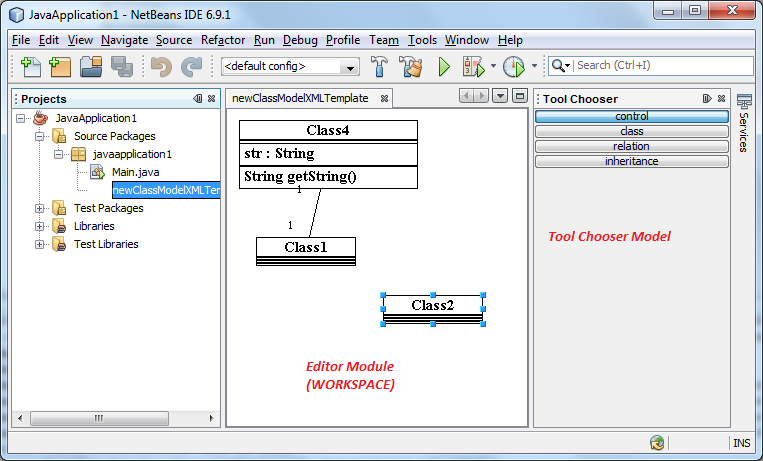
\includegraphics[width=\textwidth]{img/screenSmall.png}
\caption{Screenshot of the program}
\label{f-screenSmallModule}
\end{center}
\end{figure}

Indepmod Class Notation plugin consists of several modules which provides this functionality. The plugin is divided into modules because some parts (e.g. API of the plugin) should be public and some parts shouldn't. Public module means that it can be used in other plugins (or other modules of a plugin). These modules are:

\begin{itemize}
	\item Editor - the main module of the Indepmod Class Notation plugin. This module takes care about whole class modeling. It is used as a workspace and its user interface can be seen in the Figure \ref{f-screenSmallModule} between Project Tree and Tool Chooser panels. The workspace has a JGraph inside which controls whole class modeling.
    \item API - this module provides a public API (interfaces). Implementations of these interfaces can be found (e.g. by other Netbeans plugins) in the Lookup of the workspace (part of the Editor module). This module is public so it can be used (imported as a library) by any other plugin.
    \item Tool Chooser - is used for setting of demanded Tool of actual selected workspace. The module has a panel with single tools - e.g. Class or Relation between classes. This module will be called only ToolChooser for simplicity.
    \item JGraph - this module is used as a library wrap for JGraph (it allows other modules to use JGraph framework).
\end{itemize} 

Figure \ref{f-Editor_ToolChooser_Components} illustrates the relation between Editor and ToolChooser modules. Editor provides instances of ToolChooserModel and IClassModelModel. These interfaces can be used by other plugins/modules. One (and maybe the once at present) of these modules is ToolChooser which uses ToolChooserModel to set the desired tool of active workspace (Editor module). These interfaces will be described in detail in following section.

\begin{figure}[!ht]
\begin{center}
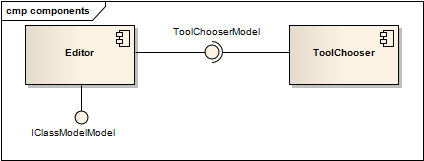
\includegraphics{img/Editor_ToolChooser_Components.png}
\caption{Component diagram of Editor and ToolChooser Modules}
\label{f-Editor_ToolChooser_Components}
\end{center}
\end{figure}

\subsection{API Module}

This module consists of interfaces (or classes) whose implementations can be found in the lookup of the workspace (workspace is the part of the editor module). This module is public so it can be used by any other module (or any other plugin). There are two packages in this module:

\begin{itemize}
    \item cz.cvut.indepmod.classmodel.api.model
    \item cz.cvut.indepmod.classmodel.api.toolchooser
\end{itemize}

\subsubsection{ClassModel API}

This package contains interfaces whose implementation can be used to access the information about class model. Lookup of the workspace contains the implementation of the IClassModelModel interface. This object provides the information about the type of a model (business model / class model) and list of classes from the model (IClass interface). Classes provides the list of annotations (IAnotation interface), attributes (IAttribute interface), methods (IMethod interface) and relations to other classes(IRelation interface). And so on with the attributes, etc. 

Relation between (two) classes is represented by instance of IRelation interface. IClass returns the list of IRelations that belongs to it. IRelation holds information about its type (simple relation, composition, agregation, generalization, implementation) and about what class is at the beginning and at the end of the relation, including cardinalities. 

Cardinalities are represented by instance of ICardinality interface. The ICardinality interface has two methods (getFrom() and getTo()) which return from and to value (both are of integer type). Sign of infinity (e.g. in the 1..* or * cardinality) is treated as -1. In the Table \ref{tab:cardinalityExamples} you can see examples of return values of some cardinalities.

\begin{table}[!ht]
\begin{center}
\begin{tabular}{|l|c|c|}
	\hline
	{ \bf Cardinality } & { \bf getFrom() result } & { \bf getTo() result } \\
	\hline \hline
	0 (or 0..0)      & 0 & 0  \\
	1 (or 1..1)      & 1 & 1  \\
   4 (or 4..4)      & 4 & 4  \\
	* (or 0..*)      & 0 & -1 \\
	1..*             & 1 & -1 \\
   0..1             & 0 & 1  \\
   2..5             & 2 & 5  \\
	\hline
\end{tabular}
\caption{Examples of cardinalities}
\label{tab:cardinalityExamples}
\end{center}
\end{table}

The ClassModel API can be treated as a tree. The root node of the tree is IClassModelModel instance whose children are classes, etc. In the Figure \ref{f-classApiTree} you can see the example of Class Model (on the top of the figure) and its API Tree.

\begin{figure}[!ht]
\begin{center}
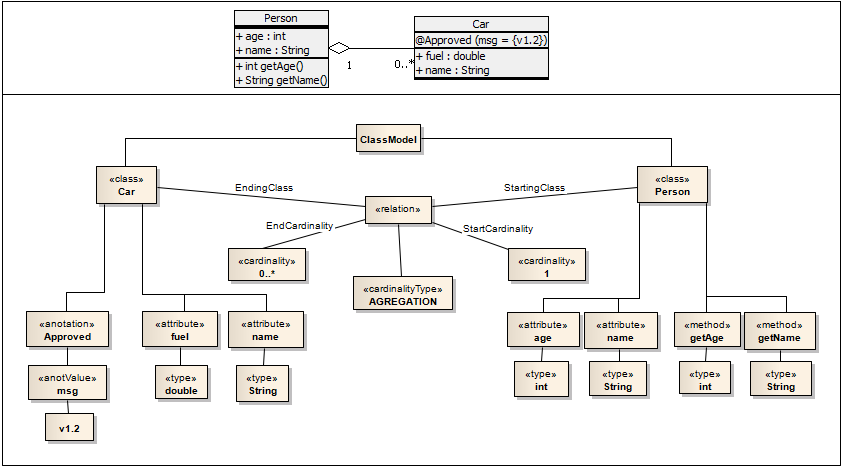
\includegraphics[width=\textwidth]{img/classModelAPITree.png}
\caption{Example of ClassModel API Tree}
\label{f-classApiTree}
\end{center}
\end{figure}

\subsubsection{ToolChooser API}

The main part of this module is ToolChooserModel class. Instance of this class represents the actual selected tool. ToolChooserModel implements the Observer design pattern so you can register your listener which will be called anytime the model changes.

This package is used by both ToolChooser and Editor modules. Workspace (part of Editor Module) has an instance of ToolChooserModel in it's lookup. This means that Editor module leaves the tool selection on someone else.

That someone else is at present ToolChooser. ToolChooser uses this instance (from the lookup of active workspace) to set the desired tool (e.g. new class).  But it is also possible to make another plugin that will do this (e.g. in the toolbar). Structure of this package is really simple and you can see it in the Figure \ref{f-ModuleAPIToolChooserModel}.

\begin{figure}[!ht]
\begin{center}
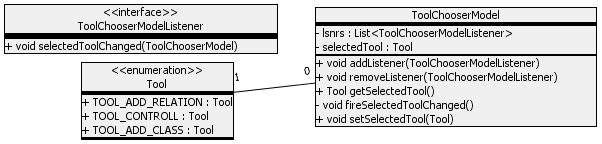
\includegraphics[width=\textwidth]{img/ModuleAPIToolChooserModel.png}
\caption{Class Diagram of ToolChooser API package}
\label{f-ModuleAPIToolChooserModel}
\end{center}
\end{figure}

\subsection{ToolChooser Module}

This module is used for setting of demanded tool of active workspace. The user interface of this module can be seen in the screen shot of the running application (Figure \ref{f-screenSmallModule}).

ToolChooser searches for instance of the ToolChooserModel in the lookup of active workspace (Editor module). When the instance is found, ToolChooser can set its tool (new class, new relation, etc.). This means that it can be used to set the desired tool of that workspace. The structure of this module can be seen in the Figure \ref{f-ToolChooserModuleToolChooser}.

\begin{figure}[!ht]
\begin{center}
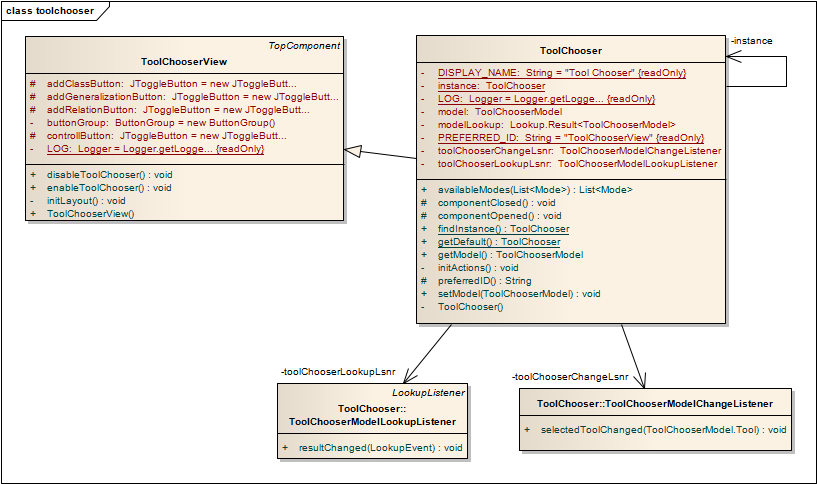
\includegraphics[width=\textwidth]{img/ToolChooserModuleToolChooser.png}
\caption{Class Diagram of ToolChooser Module}
\label{f-ToolChooserModuleToolChooser}
\end{center}
\end{figure}

ToolChooser is a singleton which is inherited from the TopComponent class. TopComponent is provided by Netbeans platform. It is derived from standard JComponent class (javax.swing) and adds many methods which can be used for controlling a window. Ancestors of TopComponent class can be used as a user interface (component that is visible to the user) in the Netbeans platform application. More info can be found in \cite{netbeans6.9DevGuide} in chapter called Window System).

In the layer.xml file there is set the action for opening the ToolChooser (in running application can be accessed in menu Windows \ding{221} Tool Chooser). Layer.xml is a configuration file of the Netbeans platform, which is provided by modules. Content of this file defines new folders and files which will be inserted into the system filesystem (a central registry) when the module is loaded. The system filesystem is a virtual filesystem, which is used for Netbeans platform settings. For example there are some folders that are used for Window System API (window positions, etc.) or Actions API (e.g. actions in the menu) configuration. More info about this can be found in \cite{netbeans6.9DevGuide} in the chapter 3, called Window System.

\subsection{Editor Module}

This is the fundamental module whose purpose is to create a workspace which provides the class modeling. For graphical part of class modeling is used framework JGraph (http://www.jgraph.com/). More info about JGraph framework can be found in \cite{jgraphmanual}.

\subsubsection{Module Structure}
\label{section:editorModuleStructure}

Main class (part of the cz.cvut.indepmod.classmodel.workspace package), which comprises the workspace, is the ClassModelWorkspace. Thus, if you want to study the code, you should start right here. ClassModelWorkspace is extended from the TopComponent. This class is responsible for whole initialisation. It creates:
\begin{itemize}
    \item ClassModelGraph - this class is extended from JGraph and represents the class model graph to the user. Instance of this class is situated inside the ClassModelWorkspace component (JGraph is also derived from JComponent)
    \item ClassModelModel - Implementation of IClassModelModel which returns the list of classes that are in the class model and the type of the diagram (class or business model).
    \item ClassModelMarqueeHandler - this class is responsible for user input handling which is made inside the ClassModelGraph.
\end{itemize}

ClassModelWorkspace is simply JComponent (TopComponent) which has the JGraph inside. JGraph presents the class model to the user. There are cells (representing classes) which are related together by edges (representing relations).

In next section I will try to describe the implementation of the Editor Module. I Will start from the initialization and after that I will try to explain every part that is created during the initialization.

\subsubsection{Editor Module Initialisation}

As I have already said before, the ClassModelWorkspace class do the initialization of the whole module. There are two cases of initialization. The first case, when user creates new class diagram, and the second, when user opens an existing model from file. Both cases are very similar. They differ in the way of ClassModelDiagramDataModel initialization. For this purpose there are two constructor variants.

ClassModelDiagramDataModel class represents the data which has to be persisted when user want to save his class diagram. At present, instance of this class holds the GraphLayoutCache instance (class of JGraph framework which holds the information about cells in the graph), list of static data types (default list of data types for certain language which is chosen during new class diagram file creation) and the type of the diagram (class or business model, it is also chosen during new file creation).

The first, non parametric, constructor is used when the new class diagram (with no associated file) is created. This constructor calls the ClassModelDiagramModelFactory which creates new instance of ClassModelDiagramDataModel and returns it.

The second constructor is used when the user opens a file with a class model. It accepts an instance of ClassModelXMLDataObject (one parameter). This object represents the file in which is the class model saved (more in the chapter \ref{subsection:fileAssociation}). The constructor gets the input stream of that file and asks the ClassModelXMLCoder to decode its content. ClassModelXMLCoder decodes it and returns ClassModelDiagramDataModel instance filled according to that file's content. ClassModelXMLCoder is part of the persistence layer and will be discussed in the chapter \ref{subsection:persistence}.

After the ClassModelDiagramDataModel is gained (created or loaded) the initialization is the same. What the ClassModelWorkspace creates have been already written up in chapter \ref{section:editorModuleStructure}. For better understanding you can see the sequence diagram in the Figure \ref{f-ClassModelWorkspaceInicializationSimple} which shows the initialisation of new ClassModelWorkspace. For simplicity there is only what ClassModelWorkspace creates. The processes inside these classes are not shown (Sequence diagram would have been really big) but the process of creation will be discussed later.

\begin{figure}[!ht]
\begin{center}
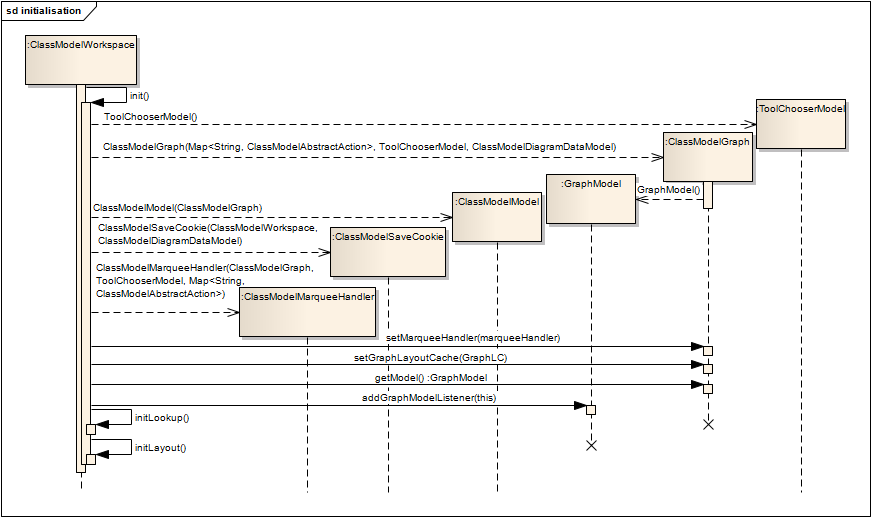
\includegraphics[width=\textwidth]{img/ClassModelWorkspaceInicializationSimple.png}
\caption{Simplified sequence diagram of ClassModelWorkspace initialization}
\label{f-ClassModelWorkspaceInicializationSimple}
\end{center}
\end{figure}

\subsubsection{Netbeans File Association}
\label{subsection:fileAssociation}

Netbeans platform allows its plugins to recognize new types of files. So when you want to associate new file type with your plugin, you can do it easily. If you are not familiar with this, you can find it in \cite{netbeans6.9DevGuide} in the chapter called Data System.

The file type association settings can be found in layer.xml file. At present there is settings of file type association and settings of wizard that can be used to create new class diagram file. In this wizard user sets the name of the file, type of the diagram and the language (Java, C++, etc.). Files that are associated with this plugin are XML files with .cls suffix. Content of these files will be discussed later.

\subsubsection{ClassModelGraph implementation}

ClassModelGraph is extended from JGraph, which provides a lot of useful functionality (more on this can be found in \cite{jgraphmanual}). ClasModelGraph adds some functionality for class manipulation. This added functionality is shown in following list.
\begin{itemize}
    \item insertCell(Point p) - creates new cell on desired position according to the selected tool (in ToolChooserModel). Usage of this function is shown in the section \ref{subsection:apiImplementation} in Figure \ref{f-ClassCreationSequenceDiagram}.

    \item getAllClasses() - returns the list of classes that are in the diagram. Usage of this function will be shown in the section \ref{subsection:apiImplementation}

    \item getAllTypes() - returns the list of all data types in the diagram. In addition to the classes (the class is a data type) there are also static data types (like String or int in Java).
\end{itemize} 

To handle events in the graph (ClassModelGraph) there is the ClassModelMarqueeHandler. Instance of this class is created in the ClassModelWorkspace and is added into the ClassModelGraph instance. Purpose of this class is to handle all user inputs in the ClassModelGraph (in the canvas of the graph) and control the popup menu (JPopupMenu and its content). When user does an action (e.g. click with mouse), the ClassModelMarqueeHandler will find out if it is a control click (e.g. cell selection), new cell addition, edge (line between cells) addition and so on. This class is also responsible for rendering of the temporary line when user creates new edge.

\subsubsection{JGraph class cell rendering}

In this section I will explain how I render the class (the rectangle with the class name and lists of annotations, attributes and methods) into the JGraph workspace. But first a little theory remind. JGraph uses MVC pattern for cell rendering. Cells (the model of cell) in JGraph are represented by DefaultGraphCell (or its subclasses). DefaultGraphCell implementation stores the user object and an attribute map. This map is used when you want to set the appearance of that cell. All graph cell has an associated view (VertexView implementation). This VertexView implementation associates the renderer, editor and cell handle\footnote{Cell handle is what appears when the cell is selected (e.g mouse click) and what allows to resize it.} together for a cell (DefaultGraphCell implementation). The cell and the view is associated together by CellViewFactory which returns a cell view for a particular cell. More on this theme can be found in \cite{jgraphmanual}.

JGraph basically supports rendering of basic shapes like rectangles, ovals and so on. When you want to render your own shape, you have to create your own cell view (VertexView), renderer (CellViewRenderer) and CellViewFactory implementation.

So this is what I did. I created ClassModelCellViewFactory which is derived from JGraph's DefaultCellViewFactory and overrides it's method createVertexView(Object o). If the object in the parameter is instance of ClassModelClassCell class, the method returns new instance of ClassModelVertexView (derived from JGraph's VertexView). Otherwise the method returns the default view (calls its parent's method). ClassModelVertexView returns instance of ClassModelVertexRenderer which is derived from VertexRenderer. ClassModelVertexRenderer overrides its method getRendererComponent. This method returns new instance of ClassComponent. ClassComponent is extended from JComponent and renders the class according to the ClassModel user object.

These classes can be found in the package cz.cvut.indepmod.classmodel.workspace.cell. Instance of ClassModelCellViewFactory is inserted into the GraphLayoutCache during the workspace initialisation. You can see the class diagram in the Figure \ref{f-ClassModelVertexStructure}.

\begin{figure}[!ht]
\begin{center}
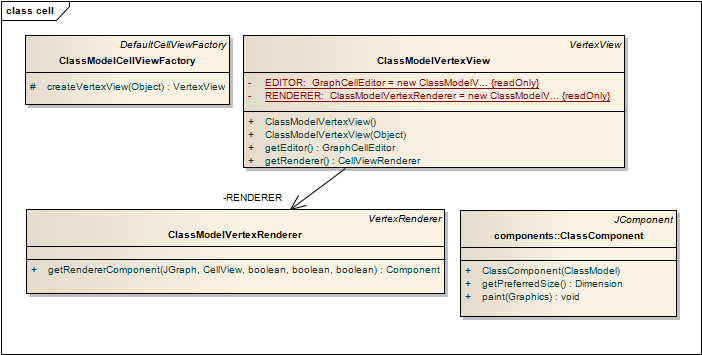
\includegraphics[width=\textwidth]{img/ClassModelVertexStructure.png}
\caption{Structure of classes which render the class cell}
\label{f-ClassModelVertexStructure}
\end{center}
\end{figure}

\subsubsection{ClassModel API implementation}
\label{subsection:apiImplementation}

Implementation classes of ClassModel API (its interfaces are in the API Module) are situated in the cz.cvut.indepmod.classmodel.cell.model.classmodel package. Main problem I had to deal with was to design where to store the data of the ClassModel.

Basically, ClassModel class is used as a User Object for JGraph cells. User Object (Class Model instance) does not have normally the pointer to its cell (only cell has the pointer to it's User Object). ClassModel holds information like name of the class and list of its attributes, methods and annotations. But where to store the information about relations with other cells (classes)? This information is stored in the JGraph (in its model). So the first idea was to copy this information into the ClassModel instance when an relation is created. But this is not very nice because of data duplication. The second purpose was to add an pointer to cell into the ClassModel instance. But how? The answer is quite simple. I created the ClassModelClassCell which extends DefaultGraphCell of JGraph. The extension of this class is that it adds an pointer to itself into the User Object if this User Object is instance of ClassModel.

So problem is solved. Some information like the name are stored inside the User object and some like the relations are gained from the JGraph cell. In the Figure \ref{f-ClassCreationSequenceDiagram} you can see how is created a class when user selects new class tool in the ToolChooser and clicks somewhere in the ClassModelGraph (JGraph) workspace.

\begin{figure}[!ht]
\begin{center}
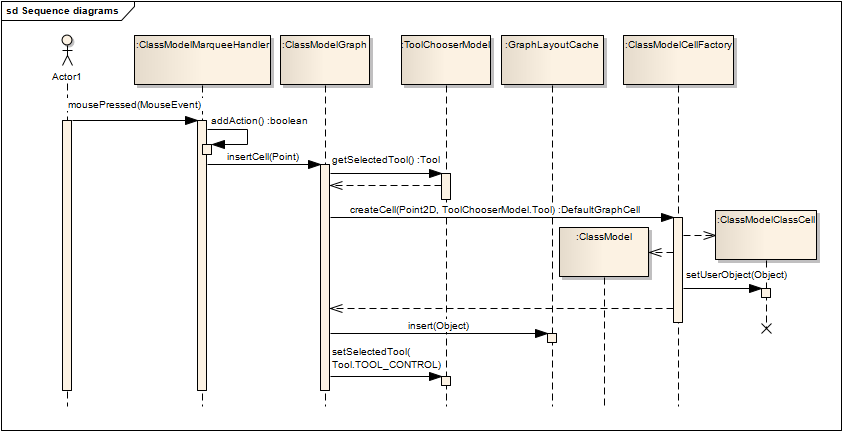
\includegraphics[width=\textwidth]{img/ClassCreationSequenceDiagram.png}
\caption{Sequence Diagram of class creation}
\label{f-ClassCreationSequenceDiagram}
\end{center}
\end{figure}

\subsubsection{Persistence}
\label{subsection:persistence}

Persistence layer implementation is situated in the cz.cvut.indepmod.classmodel.persistence.xml package. There is a ClassModelXMLCoder class that is created as a singleton. Instance of this class is responsible for encoding and decoding the ClassModelDiagramDataModel instance into or from a stream (InputStream or OutputStream). Its method for encoding, encode(ClassModelDiagramDataModel model, OutputStream stream), is called by SaveCookie (discussed in the section \ref{subsection:lookup}).

ClassModelXMLCoder uses java.beans.XMLEncoder and java.beans.XMLDecoder. This creates the xml file that represents the steps to create the exactly same object that was encoded. Because XMLEncoder can encode in default only some types of objects, there are some persistence delegates that allow to encode particular object I use. These persistence delegates can be found in the cz.cvut.indepmod.classmodel.persistence.xml.delegate package.

If you want to know more about how XMLEncoder or XMLDecoder works, please take a look at \cite{usingXMLEncoder}.

\subsubsection{Lookup}
\label{subsection:lookup}

Lookup is (in Netbeans platform) a technique to join more plugins together with loose coupling. On the module level, lookups enable to register a service by its provider and find the service by its consumer in a central repository. On the level of single components (TopComponent), lookups enable to exchange data between this component (provider) and consumers. The main difference between lookup on the module level (service registry) and lookup on the component level is that component does not provide its data by a central registry but by its own lookup object. More reading about this can be found in \cite{netbeans6.9DevGuide} in the chapter called Lookup.

Editor Module uses the Lookup on the component level. ClassModelWorkspace creates its Lookup during the initialization. It adds there an instance of ToolChooserModel and an instance of ClassModelModel.

ToolChooserModel instance is used by ToolChooser Module to set the desired tool. Thanks to this, there can be one ToolChooser component which manages all ClassModelWorkspaces. Of cource, ToolChooserModel instance in the lookup can be used by other plugins also.

ClassModelModel instance implements the IClassModelModel interface and can be also used by other plugins. It provides the Class Model API to the outside world. Thanks to this there can be for example another plugin that will generate the code from the class model of this module.

When user does any change into the model (add new class, new relation between classes, change the attribute of the class or something similar), ClassModelWorkspace inserts a SaveCookie instance into its Lookup. This tells the Netbeans platform that this component is changed and can be saved (save action in File menu is enabled). When user calls this action, the SaveCookie tells the ClassModelXMLCoder to save the GraphLayoutCache into the associated file. When it is done, this SaveCookie implementation is removed from the Lookup, so the Netbeans platform knows that the component does not have to be saved.

\subsubsection{Package Structure}

You can see the package structure in this directory tree:
\renewcommand*\DTstylecomment{\rmfamily\color{black}\textsc}
\renewcommand*\DTstyle{\ttfamily\textcolor{blue}}
\dirtree{%
.1 cz.cvut.indepmod.classmodel.
.1 actions\DTcomment{Actions for buttons etc.}.
.1 file\DTcomment{SaveCookie and file type association support}.
.2 wizard\DTcomment{Wizard for creation of new class model file}.
.1 frames.
.2 dialogs.
.1 modelfactory.
.2 diagrammodel.
.1 persistence\DTcomment{layer for data saving}.
.2 xml\DTcomment{implementation of persistence for saving into a XML file}.
.3 delegate\DTcomment{XML Delegates for mapping into xml}.
.1 resources.
.1 util.
.1 workspace\DTcomment{Main package containing the TopComponent with JGraph}.
.2 cell\DTcomment{Cells, renderers, VertexViews, etc. for JGraph}.
.3 components\DTcomment{Component for JGraph}.
.3 model.
.4 classmodel\DTcomment{Implementation of ClassModel API from API Module}.
}
\parindent=\luckyparindent

\begin{thebibliography}{9}
\bibitem{jgraphmanual}{\it{JGraph 5 manual} [online]. 2009-09-25 [cit. 2011-03-03]. Available from WWW: \url{http://www.jgraph.com/downloads/jgraph/jgraphmanual.pdf}.}

\bibitem{netbeans6.9DevGuide}{PETRI, J�rgen. \it{NetBeans Platform 6.9 	Developer's Guide}. Birmingham : Packt Publishing Ltd., 2010. 273 s. ISBN 978-1-849511-76-6}

\bibitem{usingXMLEncoder}{MILNE, Philip. \it{Sun Developer Network} [online]. 2010 [cit. 2011-01-29]. Using XMLEncoder. Available from WWW: \url{http://java.sun.com/products/jfc/tsc/articles/persistence4/}.}

\bibitem{netbeansWebNewFileTemplate}{\it{Netbeans Platform} [online]. 2005-06-26, 2008-04-15 [cit. 2011-03-03]. NetBeans File Template Module Tutorial. Available from WWW: \url{http://platform.netbeans.org/tutorials/60/nbm-filetemplates.html}.}

\bibitem{netbeansWebWizardNewFile}{\it{Creating a Better Java Class Wizard} [online]. 2008-04-02 [cit. 2011-03-03]. Geertjan's Blog. Available from WWW: \url{http://blogs.sun.com/geertjan/entry/creating_a_better_java_class}.} %Wizard for creation of new file
\end{thebibliography}

\end{document}

\end{document}

